\documentclass[12pt]{article}%12-point font
\usepackage[utf8]{inputenc}
\usepackage{amsmath}
\usepackage{amssymb}
\usepackage{mathabx}
\usepackage{graphicx}
\usepackage{subfig}
\usepackage{hyperref}
\usepackage{siunitx}
\usepackage{commath}
\usepackage{xcolor}
\usepackage{tkz-euclide} %  https://www.mathcha.io/ generates TeX figures 
\usepackage{braket} 
\usepackage{fullpage}%this sets the margins to 1 inch
\usepackage{pifont}
\newcommand{\cmark}{\ding{51}}%
\newcommand{\xmark}{\ding{55}}%
\usepackage{epigraph}
\usepackage{setspace}
\renewcommand{\baselinestretch}{1.5} %this sets the default spacing to 1.5

\begin{document}
\begin{center}
\begin{large}
\textbf{Theoretical analysis of ultrasonic vortex beam generation with single-element transducer and phase plate}\\ %update I prefer not capitalizing every letter. Are you ok with this, Yuqi?
\end{large}
\textbf{Chirag Gokani, Yuqi Meng}
\end{center}
{\setstretch{1.0}
\epigraph{Going on means going far\\ Going far means returning}{Tao Te Ching}
}


\section*{Abstract} %update

The pressure field of a vortex beam generated by a single-element transducer and phase plate is calculated, replicating the theoretical results presented in \cite{ref1} by Terzi et al. Their discussion is extended with Fraunhofer and Fresnel analyses, for which analytical expressions of the pressure magnitude and phase are obtained. Applications of vortex beams will also be described. %If time permits, a finite element method (FEM) solution will be sought to validate the analysis. A parameter optimization may also be discussed. %update

Section (\ref{Problem}) outlines the problem and defines coordinates and parameters. Section (\ref{Rayleigh integral solutions}) expresses the pressure field solution in terms of the first and second Rayleigh integrals. Section (\ref{Numerical integration}) outlines how these integrals are computed numerically. Sections (\ref{Fraunhofer limit}) and (\ref{Fresnel limit}) respectively assess the Fraunhofer and Fresnel limits. Finally, section (\ref{Applications}) offers a larger perspective on vortex beams. The \href{https://github.com/cag170030/Ultrasonics_2022}{supplemental notes} are mainly pedagogical,  deriving equations that are assumed in the literature. To match Terzi et al., the $e^{-i\omega t}$ time convention is used in this work. %update ...Is there a better place to put this information?


\section{Outline of the problem}\label{Problem}

To generate a vortex beam, Terzi et al.  impart angular momentum to a propagating sound wave. The propagating sound wave is generated by a \color{magenta}single-element transducer\color{black}, and the angular momentum is imparted using a \color{blue}phase plate\color{black}. Figure (\ref{geometry}) shows the arrangement of these elements, and table (\ref{geometrytable}) provides their positions along the $z$-axis. The source and background material properties are provided in table (\ref{materialtable}). 


\begin{table}
\centering
\begin{tabular}{ r | l | r } 
 \textbf{Variable} & \textbf{Description} & \textbf{Value} (mm)\\
 \hline
 $z_{00}$ & transducer depth & 13.4\\
 $z_{01}$ & distance from phase plate to outer edge of transducer & 10\\
 $z_{1}$ & distance from center of transducer to phase plate & 23.4\\
 $z_{0}$ & distance from center of transducer to plane of observation & 100
\end{tabular}
\caption{Given above are the positions of elements as reported in Terzi et al., measured from $z=0$ along the $z$-axis. Note that $z_{00} + z_{01} = z_1$.}\label{geometrytable}
\end{table}


\begin{table}
\centering
\begin{tabular}{ r | l | r l } 
 \textbf{Variable} & \textbf{Description} & \textbf{Value} & \textbf{Dimensions} \\
 \hline
 $F$ & surface curvature radius of transducer& 100\\
 $D$ & diameter of transducer & 100\\
 $f$ & drive frequency of transducer & 1.092 & MHz\\
 $\rho_0 $ & density of water & 1000 & kg/m$^3$\\
 $c_0$ & speed of sound in water & $1481 $ & m/s
\end{tabular}
\caption{The geometric and physical properties of transducer and background medium are given above.}\label{materialtable}
\end{table}


\iffalse
$R$ &  & distance from $\dif S$ to point of observation\\
 & $\neq e^{j\omega t}$!!& time convention\\
$\varphi$ & $=\arctan (y/x)$ & polar angle\\
$l$& $=0,1,2,\dots$ & orbital number\\
\fi


%Description of transducer
%Description of phase plate
The \color{magenta}transducer \color{black}  lies in the $z=0$ plane and pulsates at frequency $f$ (corresponding to wavenumber $k = 2\pi f/c_0$) in the $z$-direction with vibration velocity amplitude $V$. The surface of the transducer is denoted by \color{magenta}$S_0$\color{black}, and a differential element of this surface is given by \color{magenta}$\dif S_0$\color{black}. The distance from the transducer surface to a point of observation $(x,y,z) \equiv \boldsymbol r$ is given by \color{magenta} 

$$R = \sqrt{(x-x_0)^2 + (y-y_0)^2 + z^2}.$$

\color{black}Meanwhile, the \color{blue}phase plate \color{black}  lies at $z = z_1 = z_{00} + z_{01}$, contributing vorticity to the pressure field generated by the transducer. Physically, the vorticity is achieved by varying the phase plate's thickness over the polar angle $\varphi \equiv \arctan (y/x)$; the incident sound accumulates a local phase depending on the thickness of the plate through which it passes. Mathematically, the vorticity contributes a factor of ${e}^{i\Phi(\varphi) }$ to the complex-exponential form of solution. Since vortex beams are by definition helices that repeat their angular behavior over many cycles in $\varphi$, $e^{i\Phi(\varphi)}$ must be either constant or periodic in $2\pi/l$, where $l=$ the orbital number $=1,2,\dots$. That is, 

\begin{align*}
    e^{i\Phi(\varphi)} &= \begin{cases}
    1, \text{ \space constant} \\    
  e^{i\phi l}, \text{ \space periodic in $2\pi/l$}
  \end{cases}\\
  \implies \Phi(\varphi) &= \begin{cases}
      0, \text{ \space constant} \\    
 l \varphi, \text{\space where } l=\pm1,\pm2,\dots, \text{ \space periodic in $2\pi/l$}
  \end{cases}
\end{align*}

\noindent The two cases above can be combined as $\Phi (\varphi) = l\varphi$ and letting $l = 0, \pm1, \pm2,\dots$. A vortex beam that is continuous along $\varphi$ is achieved in the $l\to\infty$ limit, while a vortex beam that has $l$ modes of equal phase requires $l$ sectors on the phase plate. Terzi et al. note that this behavior is difficult to achieve, however, due to fabrication limitations. This work follows suit by considering relatively low values of $l$. %update , though large $l$ cases are considered at the end of section (\ref{})
Figure (\ref{phase plate figure}) shows how the phase plate determines $l$ and offers a physical interpretation of the the orbital number.%need to complete figure for this

\begin{figure}%
    \centering
\tikzset{every picture/.style={line width=0.75pt}} %set default line width to 0.75pt        
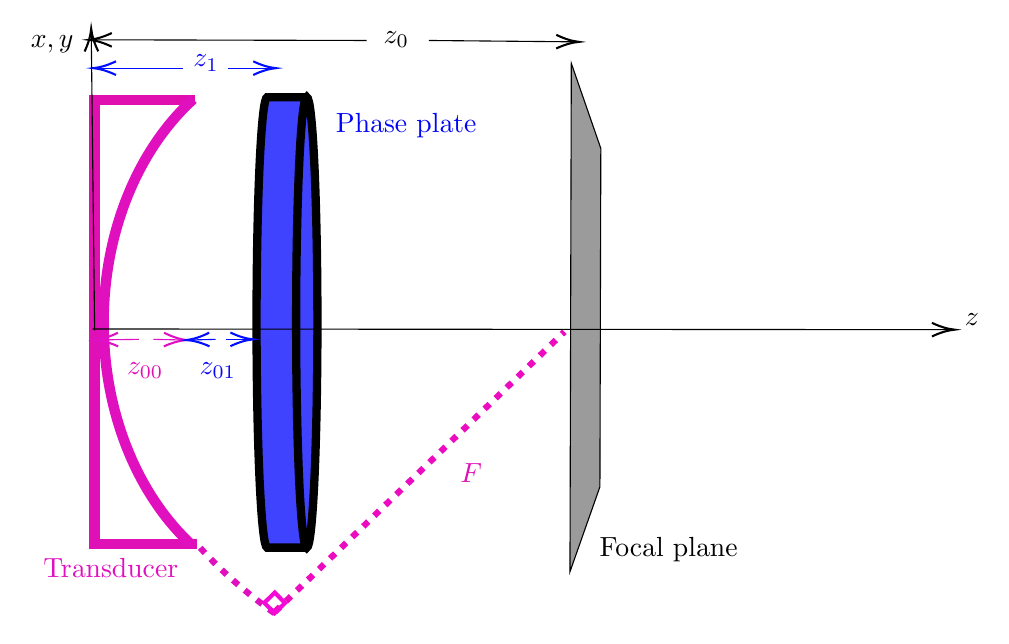
\begin{tikzpicture}[x=0.75pt,y=0.75pt,yscale=-1,xscale=1]
%uncomment if require: \path (0,354); %set diagram left start at 0, and has height of 354

%Flowchart: Direct Access Storage [id:dp022466445870493956] 
\draw  [fill={rgb, 255:red, 3; green, 8; blue, 253 }  ,fill opacity=0.76 ][line width=3]  (213.2,256.33) -- (194.13,256.33) .. controls (191.3,256.33) and (189,207.76) .. (189,147.83) .. controls (189,87.91) and (191.3,39.33) .. (194.13,39.33) -- (213.2,39.33)(218.33,147.83) .. controls (218.33,207.76) and (216.04,256.33) .. (213.2,256.33) .. controls (210.36,256.33) and (208.07,207.76) .. (208.07,147.83) .. controls (208.07,87.91) and (210.36,39.33) .. (213.2,39.33) .. controls (216.04,39.33) and (218.33,87.91) .. (218.33,147.83) ;
%Shape: Right Angle [id:dp37120949208238563] 
\draw  [color={rgb, 255:red, 224; green, 16; blue, 176 }  ,draw opacity=1 ][line width=3.75]  (111,179) -- (111,40.67) -- (159.33,40.67) ;
%Shape: Right Angle [id:dp8154955687723711] 
\draw  [color={rgb, 255:red, 224; green, 16; blue, 183 }  ,draw opacity=1 ][line width=3.75]  (111,138) -- (111,254.67) -- (160.33,254.67) ;
%Shape: Arc [id:dp9085670797872456] 
\draw  [draw opacity=0][line width=3.75]  (157.4,254.71) .. controls (131.94,230.96) and (115.33,192.01) .. (115.33,148) .. controls (115.33,103.37) and (132.41,63.94) .. (158.49,40.29) -- (215.54,148) -- cycle ; \draw  [color={rgb, 255:red, 224; green, 16; blue, 190 }  ,draw opacity=1 ][line width=3.75]  (157.4,254.71) .. controls (131.94,230.96) and (115.33,192.01) .. (115.33,148) .. controls (115.33,103.37) and (132.41,63.94) .. (158.49,40.29) ;  
%Shape: Arc [id:dp6103333919650833] 
\draw  [draw opacity=0][dash pattern={on 2.53pt off 3.02pt}][line width=2.25]  (197.66,287.94) .. controls (182.41,276.98) and (169.59,265.41) .. (160.33,254.67) -- (222,268.31) -- cycle ; \draw  [color={rgb, 255:red, 224; green, 16; blue, 190 }  ,draw opacity=1 ][dash pattern={on 2.53pt off 3.02pt}][line width=2.25]  (197.66,287.94) .. controls (182.41,276.98) and (169.59,265.41) .. (160.33,254.67) ;  
%Straight Lines [id:da4181129718985068] 
\draw [color={rgb, 255:red, 236; green, 11; blue, 191 }  ,draw opacity=1 ][line width=2.25]  [dash pattern={on 2.53pt off 3.02pt}]  (197.85,287.28) -- (337.33,152.33) ;
%Shape: Square [id:dp9017802043841254] 
\draw  [color={rgb, 255:red, 244; green, 9; blue, 214 }  ,draw opacity=1 ][line width=1.5]  (192.76,282.89) -- (197.8,277.99) -- (202.7,283.04) -- (197.66,287.94) -- cycle ;
%Straight Lines [id:da08007812146456739] 
\draw [color={rgb, 255:red, 224; green, 16; blue, 197 }  ,draw opacity=1 ]   (139.33,156) -- (153.33,156.29) ;
\draw [shift={(155.33,156.33)}, rotate = 181.19] [color={rgb, 255:red, 224; green, 16; blue, 197 }  ,draw opacity=1 ][line width=0.75]    (10.93,-3.29) .. controls (6.95,-1.4) and (3.31,-0.3) .. (0,0) .. controls (3.31,0.3) and (6.95,1.4) .. (10.93,3.29)   ;
%Straight Lines [id:da052656144089168855] 
\draw [color={rgb, 255:red, 224; green, 16; blue, 197 }  ,draw opacity=1 ]   (132.33,156) -- (117.29,156.2) -- (113.33,156.29) ;
\draw [shift={(111.33,156.33)}, rotate = 358.73] [color={rgb, 255:red, 224; green, 16; blue, 197 }  ,draw opacity=1 ][line width=0.75]    (10.93,-3.29) .. controls (6.95,-1.4) and (3.31,-0.3) .. (0,0) .. controls (3.31,0.3) and (6.95,1.4) .. (10.93,3.29)   ;
%Straight Lines [id:da9913347769877889] 
\draw [color={rgb, 255:red, 0; green, 15; blue, 255 }  ,draw opacity=1 ]   (174.33,156) -- (185.33,156) ;
\draw [shift={(187.33,156)}, rotate = 180] [color={rgb, 255:red, 0; green, 15; blue, 255 }  ,draw opacity=1 ][line width=0.75]    (10.93,-3.29) .. controls (6.95,-1.4) and (3.31,-0.3) .. (0,0) .. controls (3.31,0.3) and (6.95,1.4) .. (10.93,3.29)   ;
%Straight Lines [id:da8898501278599356] 
\draw [color={rgb, 255:red, 0; green, 15; blue, 255 }  ,draw opacity=1 ]   (169.33,156) -- (157.33,156.29) ;
\draw [shift={(155.33,156.33)}, rotate = 358.64] [color={rgb, 255:red, 0; green, 15; blue, 255 }  ,draw opacity=1 ][line width=0.75]    (10.93,-3.29) .. controls (6.95,-1.4) and (3.31,-0.3) .. (0,0) .. controls (3.31,0.3) and (6.95,1.4) .. (10.93,3.29)   ;
%Straight Lines [id:da23578248392040324] 
\draw [color={rgb, 255:red, 0; green, 15; blue, 255 }  ,draw opacity=1 ]   (175.33,25.33) -- (196.33,25.33) ;
\draw [shift={(198.33,25.33)}, rotate = 180] [color={rgb, 255:red, 0; green, 15; blue, 255 }  ,draw opacity=1 ][line width=0.75]    (10.93,-3.29) .. controls (6.95,-1.4) and (3.31,-0.3) .. (0,0) .. controls (3.31,0.3) and (6.95,1.4) .. (10.93,3.29)   ;
%Straight Lines [id:da17442533312591424] 
\draw [color={rgb, 255:red, 0; green, 15; blue, 255 }  ,draw opacity=1 ]   (153.33,25.33) -- (112.33,25.33) ;
\draw [shift={(110.33,25.33)}, rotate = 360] [color={rgb, 255:red, 0; green, 15; blue, 255 }  ,draw opacity=1 ][line width=0.75]    (10.93,-3.29) .. controls (6.95,-1.4) and (3.31,-0.3) .. (0,0) .. controls (3.31,0.3) and (6.95,1.4) .. (10.93,3.29)   ;
%Shape: Trapezoid [id:dp8510035605974002] 
\draw  [fill={rgb, 255:red, 155; green, 155; blue, 155 }  ,fill opacity=1 ] (340.65,22.99) -- (354.87,64) -- (354.44,227.02) -- (340.01,267.96) -- cycle ;
%Straight Lines [id:da4089745292378264] 
\draw    (272,12) -- (342.33,12.65) ;
\draw [shift={(344.33,12.67)}, rotate = 180.53] [color={rgb, 255:red, 0; green, 0; blue, 0 }  ][line width=0.75]    (10.93,-3.29) .. controls (6.95,-1.4) and (3.31,-0.3) .. (0,0) .. controls (3.31,0.3) and (6.95,1.4) .. (10.93,3.29)   ;
%Straight Lines [id:da11216456046884105] 
\draw    (242,12) -- (110.33,11.67) ;
\draw [shift={(108.33,11.67)}, rotate = 0.14] [color={rgb, 255:red, 0; green, 0; blue, 0 }  ][line width=0.75]    (10.93,-3.29) .. controls (6.95,-1.4) and (3.31,-0.3) .. (0,0) .. controls (3.31,0.3) and (6.95,1.4) .. (10.93,3.29)   ;
%Straight Lines [id:da6817421797910601] 
\draw    (111,151.67) -- (109.36,8.33) ;
\draw [shift={(109.33,6.33)}, rotate = 89.34] [color={rgb, 255:red, 0; green, 0; blue, 0 }  ][line width=0.75]    (10.93,-3.29) .. controls (6.95,-1.4) and (3.31,-0.3) .. (0,0) .. controls (3.31,0.3) and (6.95,1.4) .. (10.93,3.29)   ;
%Straight Lines [id:da6080898116435915] 
\draw    (110,151) -- (523.33,151.33) ;
\draw [shift={(525.33,151.33)}, rotate = 180.05] [color={rgb, 255:red, 0; green, 0; blue, 0 }  ][line width=0.75]    (10.93,-3.29) .. controls (6.95,-1.4) and (3.31,-0.3) .. (0,0) .. controls (3.31,0.3) and (6.95,1.4) .. (10.93,3.29)   ;

% Text Node
\draw (529,142.4) node [anchor=north west][inner sep=0.75pt]    {$z$};
% Text Node
\draw (79,8.4) node [anchor=north west][inner sep=0.75pt]    {$x,y$};
% Text Node
\draw (286,214.4) node [anchor=north west][inner sep=0.75pt]  [color={rgb, 255:red, 224; green, 16; blue, 181 }  ,opacity=1 ]  {$F$};
% Text Node
\draw (125.33,165.73) node [anchor=north west][inner sep=0.75pt]  [font=\normalsize,color={rgb, 255:red, 224; green, 16; blue, 181 }  ,opacity=1 ]  {$z_{00}$};
% Text Node
\draw (160.33,165.73) node [anchor=north west][inner sep=0.75pt]  [color={rgb, 255:red, 10; green, 6; blue, 243 }  ,opacity=1 ]  {$z_{01}$};
% Text Node
\draw (157.33,17.73) node [anchor=north west][inner sep=0.75pt]  [color={rgb, 255:red, 10; green, 6; blue, 243 }  ,opacity=1 ]  {$z_{1}$};
% Text Node
\draw (85,260) node [anchor=north west][inner sep=0.75pt]   [align=left] {\textcolor[rgb]{0.88,0.06,0.75}{Transducer}};
% Text Node
\draw (226,46) node [anchor=north west][inner sep=0.75pt]   [align=left] {\textcolor[rgb]{0,0.02,0.96}{Phase plate}};
% Text Node
\draw (249,6.4) node [anchor=north west][inner sep=0.75pt]    {$z_{0}$};
% Text Node
\draw (353,250) node [anchor=north west][inner sep=0.75pt]   [align=left] {Focal plane};


\end{tikzpicture}
    \caption{This schematic shows the relative positioning of the \color{magenta} transducer\color{black}, \color{blue} phase plate\color{black}, and focal plane.}%
    \label{geometry}
\end{figure}


\begin{figure}%
    \centering

    \caption{This diagrams shows how the number of sectors (denoted by ) $l=0$ mode has no vorticity, the $l= \pm1$ mode features one equal-phase surface, and higher orbital numbers each correspond to a family of $l$ helicoids.}
    \label{phase plate figure}
\end{figure}




Since a defining characterstic of the vortex beam is its radiation pattern that has vanishing on-axis intensity when projected on the transverse plane, Terzi et al. look for this feature in their model to determine the validity of their proposed vortex-beam generation method. This condition will benchmark the results presented in sections (\ref{Numerical integration}), (\ref{Fraunhofer limit}), and (\ref{Fresnel limit}).

\section{Rayleigh integral solutions}\label{Rayleigh integral solutions}

To calculate the pressure field at the focal plane, the problem is split into two parts. The first part involves calculating the pressure field generated by the \color{magenta}transducer\color{black} at $z_1^-$, where the $(-)$ superscript denotes a number infinitesimally less than $z_1$. T

\begin{equation}
p = -i \frac{\rho_0 c_0 k}{2\pi} \oiint \frac{V e^{ikR}}{R}\dif S \tag{first Rayleigh integral}
\end{equation}

and note it can be factored out of the integral because it is uniform over the surface of the source. 


\begin{equation}\label{Rayleigh 2}
p(\boldsymbol r) = \frac{1}{2\pi}\oiint_{S_1} p(\boldsymbol r_1) \frac{z_0- z_1}{R}\del{-\frac{ik}{R}+\frac{1}{R^2}} e^{ikR}\dif S
\end{equation}

The time-independent pressure for $z> 0$ therefore has the form $p(\varphi,z)e^{i\Phi(\varphi)}$. 


\section{Numerical integration of first \& second Rayleigh integrals}\label{Numerical integration}



The region of integration is a 100 mm $\times$ 100 mm square. The space is discretized using a square mesh, with side length $h = \lambda/3 = 0.5$ mm. 

\section{Fraunhofer limit}\label{Fraunhofer limit}

\section{Fresnel limit}\label{Fresnel limit}



\section{Applications}\label{Applications}



\section*{Author Contributions} %update 

C.G. and Y.M. worked together to calculate the pressure amplitude and phase distributions given by equations (1) and (2) in Terzi et al. The replication of Figure 2(a) and 2(b) were a group effort. C.G. and Y.M. worked together to seek an FEM solution to the problem.

C.G. evaluated the Fraunhofer and Fresnel limits and sought analytical solutions for the pressure amplitude and phase distributions. C.G. typed the supplementary notes.

Y.M. researched the applications of vortex beams and their relation to the larger field of ultrasonics. Y.M. modified the geometry and other relevant parameters in the FEM model to optimize its design for applications.

C.G. and Y.M. both contributed their respective sections to the report. The creation of the presentation was straightforward and was led by C.G.

\begin{thebibliography}{99}
\bibitem{ref1}
Terzi, M. E., Tsysar, S. A., Yuldashev, P. V., Karzova, M. M., and Sapozhnikov, O. A. \href{https://doi.org/10.3103/S0027134916050180}{Generation of a vortex ultrasonic beam with a phase plate with an angular dependence of the thickness}. \textit{Moscow University Physics Bulletin}. \textbf{72}, 61–67 (2017).


\bibitem{ref2}
Melde, K., Mark, A. G., Qiu, T., and Fischer, P. \href{https://doi.org/10.1038/nature19755}{Holograms for acoustics}. \textit{Nature}. \textbf{537}, 518–522 (2016).

\bibitem{ref3} 
Sallam, A., Meesala, V.C., Hajj, M.R., et al. \href{https://doi.org/10.1063/5.0065489}{Holographic mirrors for spatial ultrasound modulation in contactless acoustic energy transfer systems}.  \textit{Applied Physics Letters}. \textbf{119}, 144101 (2021).

\bibitem{ref4} 
Parker, S. \href{https://hdl.handle.net/2152/87049}{Physical limitations and practical considerations for the creation of acoustic holograms}. M.S. Thesis, The University of Texas at Austin. (2020).

\bibitem{ref5} 
Sapozhnikov, O.A., Tsysar, S.A., et al. \href{https://doi.org/10.1121/1.4928396}{Acoustic holography as a metrological tool for characterizing medical ultrasound sources and fields}. \textit{The Journal of the Acoustical Society of America} \textbf{138}, 1515 (2015). 


\end{thebibliography}
\end{document}